\documentclass[tikz,border=10pt]{standalone}
\usepackage{tikz}
\usetikzlibrary{positioning}

\tikzset{
  card/.style={draw=blue!70!black, line width=1.2pt, rounded corners=3pt, minimum width=3.4cm, minimum height=2.4cm, align=center, fill=none}
}

\begin{document}
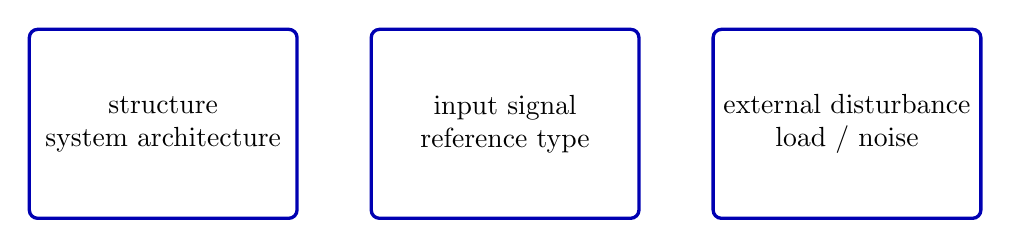
\begin{tikzpicture}[node distance=0.9cm]
  \node[card] (a) {structure\\system architecture};
  \node[card, right=of a] (b) {input signal\\reference type};
  \node[card, right=of b] (c) {external disturbance\\load / noise};
\end{tikzpicture}
\end{document}
